\chapter{Modelling of Wind Turbine Generators}

\label{ch: Mod}

With a growing share of energy covered by wind, system operators must consider how wind turbines affect the system stability during faults and maneuvers. To do so, mathematical models capable of describing these machines' behaviour are crucial. Obtaining these models, on the other hand, is not an easy task, due to considerable amount of wind turbines in large power plants, with different manufacturers, technologies, sizes, distances from point of connection and wind conditions. Thus, a model that describes well a particular turbine in a power plant, won't necessarily work for its neighboring generators. Also, due to industrial secrecy, manufacturers provide little or no information about how their turbines behave. Furthermore, having one model for every wind turbine within a power plant would result in a mathematical problem with high complexity and computational cost \cite{Erlich2012}.

\section{Generic Models of Wind Turbine Generators}

To address this problem, studies such as \cite{Muljadi2008}, \cite{Ellis2011}, \cite{council2008wecc} and \cite{Asmine2011}, motivated specially by the Institute of Electrical and Electronics Engineers (IEEE) and the Western Electricity Coordinating Council (WECC), developed generic models able to predict the behaviour of entire wind power plants. Such models reduced the problem complexity, since they were composed of a single equivalent generator. A two-machine model is needed only in rare cases, such as when the wind power plant is composed of two or more types of wind turbines \cite{Ellis2011}.

These studies have also shown that commercial wind turbine generators (WTG) could be sorted into four basic types, according to its technology \cite{Ellis2011}. These types are described in the following subsections.

\subsection{Type-1 Wind Turbine Generator}

The first type of wind turbine generator is composed of a Squirrel Cage Induction Generator (SCIG) connected to a wind turbine through a controlled gearbox, as displayed in Figure \ref{fig: WTG1}. Due to its torque-speed characteristics, generators of this type operate at constant rotor speed, requiring robust controllers on gearbox and blade. Besides, as usual to any induction generator, the SCIG absorbs reactive power during operation. Thus, capacitors are often employed for power faction correction purposes. Moreover, type-1 generators limit aerodynamic power by varying the pitch angle of their blades, imposing great mechanical stress on blades, shafts and gears, demanding a robust mechanical design and preventing these generators to operate above certain wind speed \cite{Ellis2011}. 

\begin{figure}[h]
	\caption{Representation of Type-1 Wind Turbine Generator}
	\begin{center}
		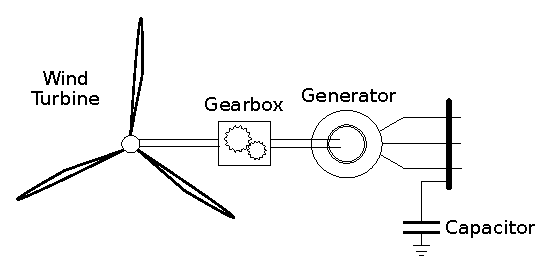
\includegraphics[scale=1]{Images/Type1WTG.eps}
	\end{center}
	\label{fig: WTG1}
\end{figure}

\subsection{Type-2 Wind Turbine Generator}

Similarly to Type-1 WTG, Type-2 Wind Turbine Generators are composed of an asynchronous machine connected to a wind turbine via gearbox, but, instead of SCIG, Wound Rotor Induction Generator (WRIG) are used to convert kinetic energy into electricity. The WRIG has access to its rotor windings, allowing to vary the rotor resistance. As a direct consequence, this machine can operate in different wind speeds by adjusting its torque-speed curve as needed \cite{Ellis2011}. Therefore, Type-2 WTG have a WRIG with a variable resistance connected to its rotor terminals, as shown in Figure \ref{fig: WTG2}.

\begin{figure}[h]
	\caption{Representation of Type-2 Wind Turbine Generator}
	\begin{center}
		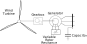
\includegraphics[scale=1]{Images/Type2WTG.eps}
	\end{center}
	\label{fig: WTG2}
\end{figure}

This type of generator has then three speed control systems, with rotor resistance control responding to rapid changes in speed, gearbox control for medium variations and pitch control for slow changes. These control system work together to maintain power output constant and reduce mechanical stress on components. The effects on the torque-speed curve caused by different rotor resistances are shown in Figure \ref{fig: Tw}. For a fixed power, increasing rotor resistance increases the speed needed on the shaft, allowing the wind turbine to operate above rated wind speed. However, the speed range is only $\pm 10\%$ of rated slip. Also, this machine still needs a reactive compensation circuit on its terminals \cite{Muljadi2010}.

\begin{figure}[h]
	\caption{Torque-speed curve}
	\begin{center}
		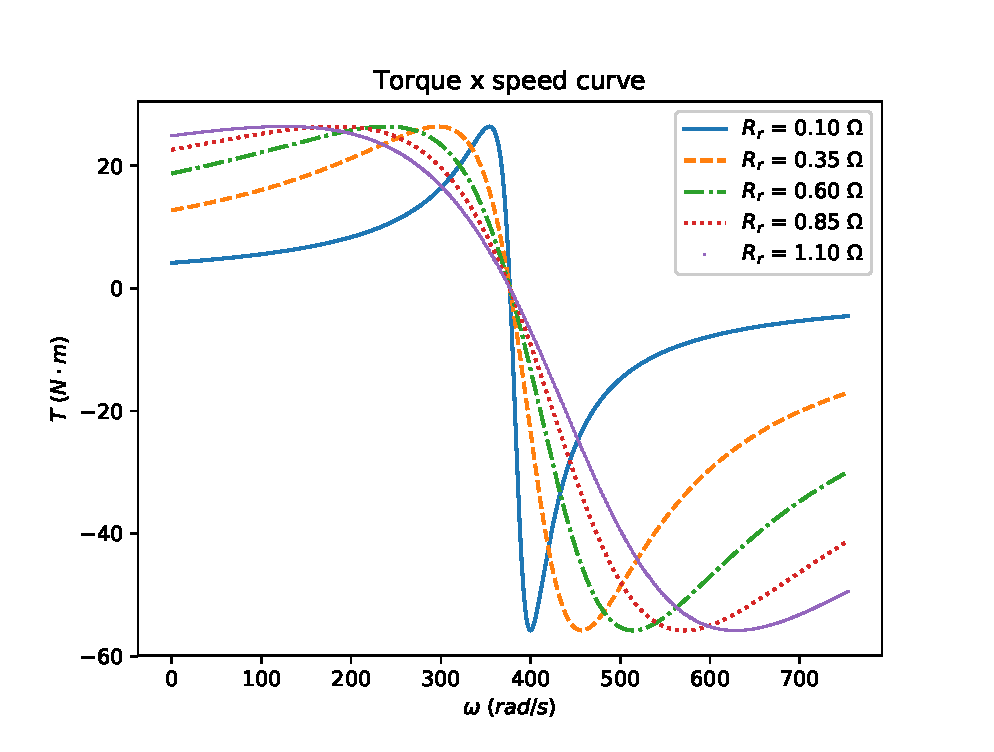
\includegraphics[scale=.7]{Images/Tw_curve.eps}
	\end{center}
	\label{fig: Tw}
\end{figure}

\subsection{Type-3 Wind Turbine Generator}

A Type-3 Wind Turbine Generator, often called Doubly Fed Induction Generator (DFIG), is also composed of a wound rotor machine connected to a wind turbine. But, instead of varying rotor resistance, a DFIG has its rotor supplied with AC voltage by a back-to-back frequency converter, as displayed in Figure \ref{fig: WTG3}. By varying the voltage frequency on the rotor circuit, the generator is able to supply power to the grid in a wider range of wind speed, reaching up to $\pm 30\%$ of rated slip. In addition, the converter can control both real and reactive power independently, ending the necessity of capacitors \cite{Muljadi2010}. Since approximately 30\% of rated power flows through the rotor windings, power electronics components have lower specifications and don't have great impact on overall costs. On the other hand, these generators need regular maintenance due to slip rings, brushes and gearbox, preventing its use in offshore applications \cite{Yaramasu2015}.

\begin{figure}[h]
	\caption{Representation of Type-3 Wind Turbine Generator}
	\begin{center}
		\includegraphics[scale=1]{Images/Type3WTG.eps}
	\end{center}
	\label{fig: WTG3}
\end{figure}

\subsection{Type-4 Wind Turbine Generator}

The last type of wind turbine generator, also called Full-Converter Generator, is composed of a electrical machine connected to the grid through a back-to-back frequency converter. The converter will operate converting the electrical frequency generated to standard, allowing this type of WTG to operate in a large range of wind speed (up to almost 100\% of rated slip). Due to the converter operation, connection to the wind turbine can be made directly or via gearbox. Likewise, it allows the use of synchronous and asynchronous electrical machines as generator, with Permanent Magnet Synchronous Generator (PMSG), Electrical Excited Synchronous Generator (EESG) and SCIG being most common, because of cost and maintenance purposes. Similar to DFIG, full-converter generators are able to control real and reactive power injected into the grid. However, since all power generated must flow through the power electronics, the overall cost of these generators is usually higher \cite{Yaramasu2015}. Figure \ref{fig: WTG4} depicts a typical Type-4 Wind Turbine Generator.

\begin{figure}[h]
	\caption{Representation of Type-4 Wind Turbine Generator}
	\begin{center}
		\includegraphics[scale=1]{Images/Type4WTG.eps}
	\end{center}
	\label{fig: WTG4}
\end{figure}

Figure \ref{fig: WindShare} shows the evolution of share in installed capacity onshore for each generator type. The data shows how SCIG and WRIG lost space in the segment and how DFIG and Full-Converter Generators' participation rose, dominating the global market \cite{Magagna2017}.

\begin{figure}[h]
	\caption{Share of installed capacity for each wind turbine generator type}
	\begin{center}
		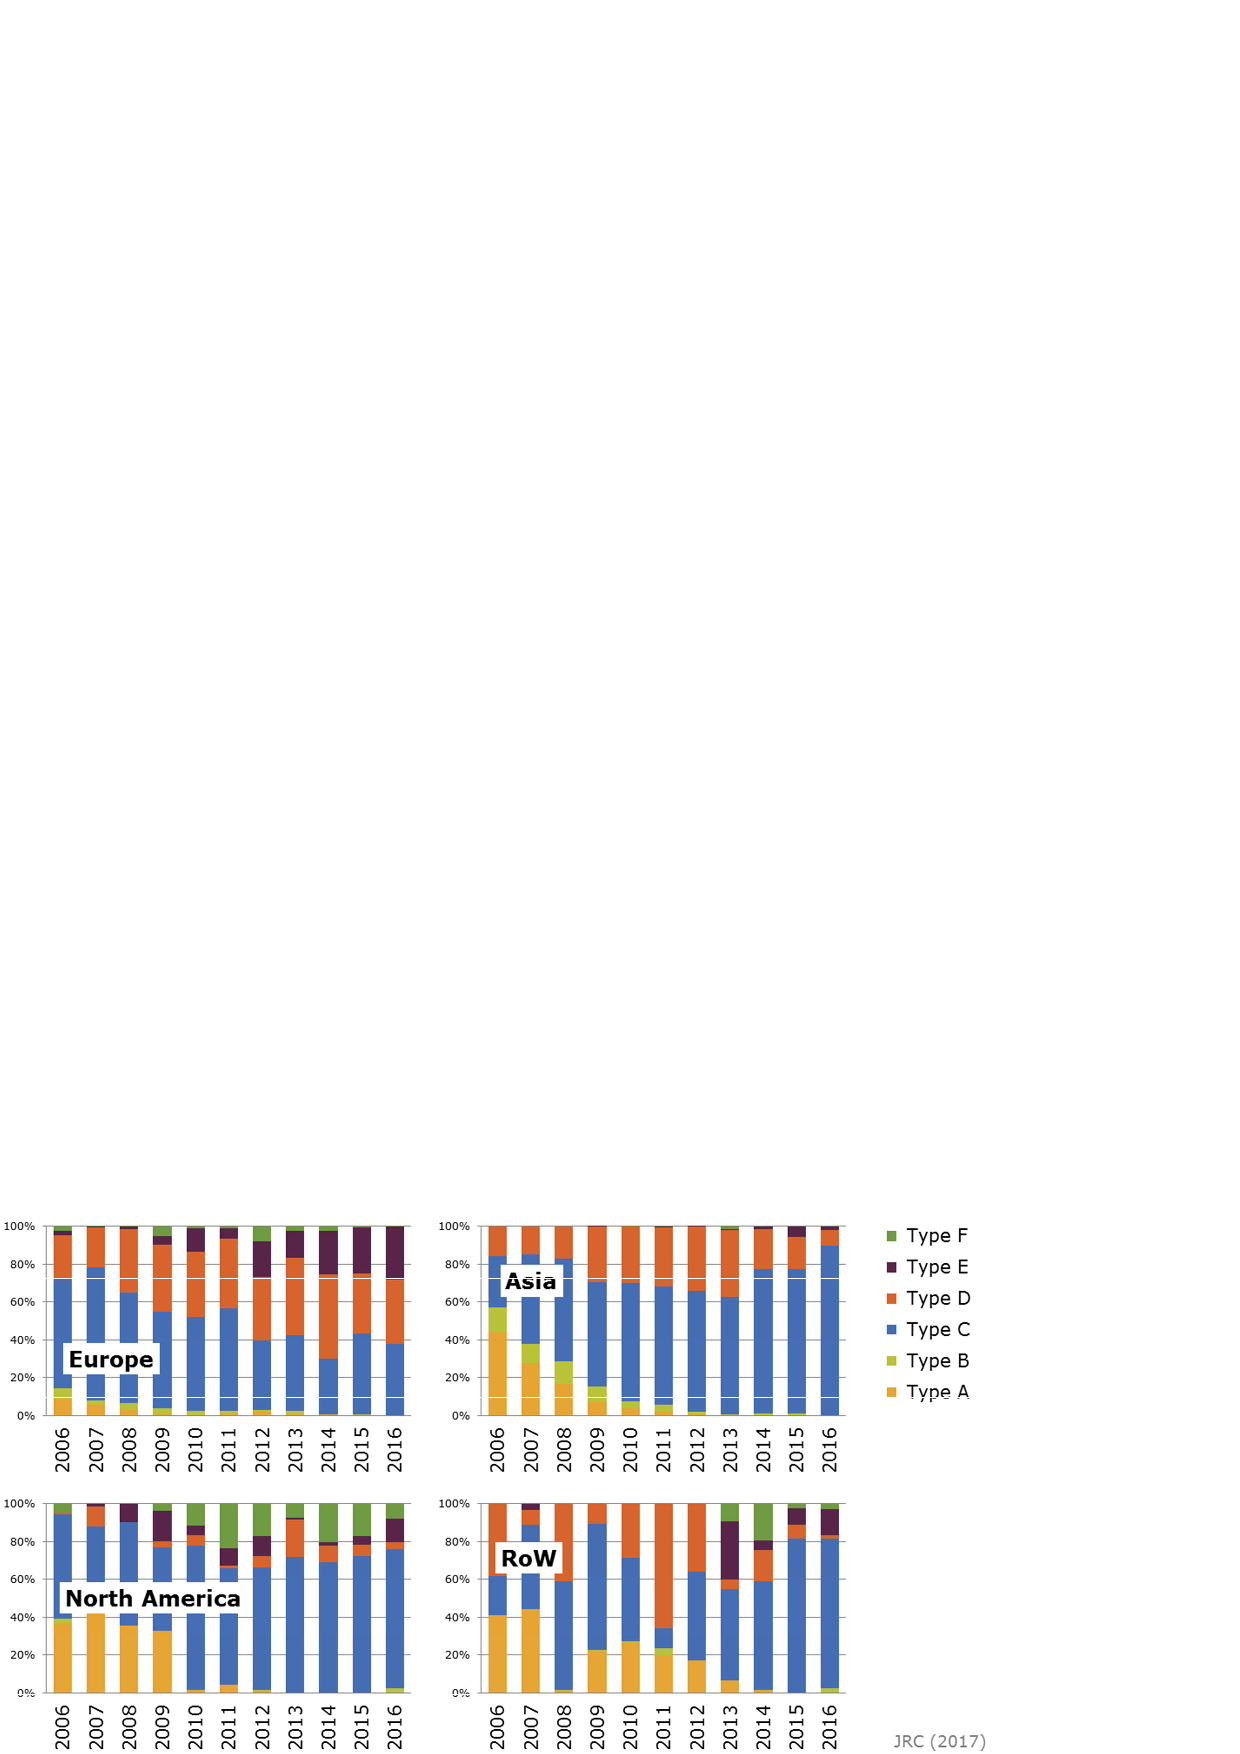
\includegraphics[scale=.2]{Images/WTGTypes.jpg}
	\end{center}
	\legend{Source: JRC}
	\label{fig: WindShare}
\end{figure}

\section{Model of Wind Turbine Generator Selected}

Many mathematical models were developed during the last years that are able to represent Wind Turbine Generators of all types. All those models have in common the fact that they are based on the generic models proposed by the studies made by WECC and IEEE and presented in the last chapter. The mathematical model selected for this work is presented in this section.

Initially proposed by \cite{Erlich2012}, the mathematical model chosen is able to represent the dynamic of both Type-3 and -4 WTG's and can be used to simulate entire wind power plants. In this model, a Thevenin equivalent circuit is connected to grid with a controlled voltage source, as depicted in Figure \ref{fig: ErlMod}. 

\begin{figure}[h]
	\caption{Type-3 WTG model proposed by Erlich}
	\begin{center}
		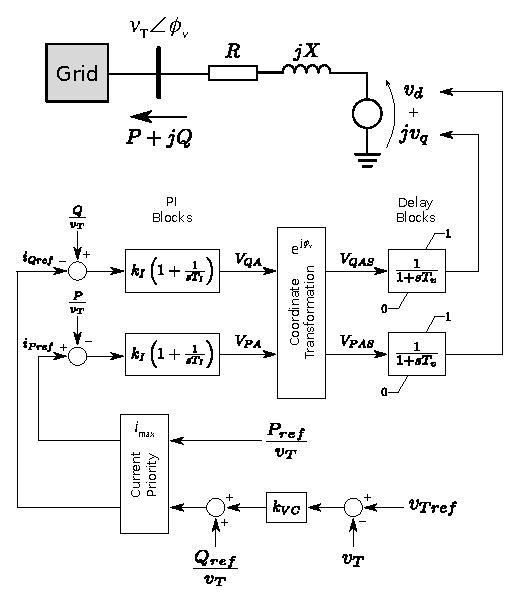
\includegraphics[scale=1]{Images/ErlichModel.eps}
	\end{center}
	\label{fig: ErlMod}
	\legend{Source: Adapted from \cite{Erlich2012}}
\end{figure}

Terminal voltage $v_{T}$ is the variable of interest in this model, appearing as input to DFIG's control system. Active and reactive current are calculated using that input, according to equation \eqref{eq: Currents}.

\begin{equation}
	\begin{cases}
		I_{Ac} = \frac{v_{T}}{p_{Tref}} \\
		I_{Re} = k_{VC}(v_{Tref} - v_{T})
	\end{cases}
	\label{eq: Currents}
\end{equation}

The calculated currents feed a current priority block. This block analyses the current magnitude and terminal voltage level and decides whether power injection or voltage control will be prioritize. In summary, it checks if the generator's current is below a maximum level $i_{max}$ and, if it is not, the block verifies if terminal voltage is above a threshold value $v^{*}$ to decide what will be prioritized. The following algorithm describes the current priority block operation.

\begin{center}
	\begin{lstlisting}[mathescape, columns=fullflexible]
	if $\sqrt{I_{Ac}^{2} + I_{Re}^{2}} \leq i_{max}$ then:
		$\begin{cases}
				i_{Pref} = I_{Ac} \\
				i_{Qref} = I_{Re}
		\end{cases}$
	else:
		if $v_{T} \geq v^{*}$ then:	
			$\begin{cases}
				i_{Pref} = min(i_{max}, I_{Ac}) \\
				i_{Qref} = \sqrt{i_{max}^{2} - i_{Pref}^{2}}
			\end{cases}$
		else:
			$\begin{cases}
				i_{Qref} = min(i_{max}, I_{Re}) \\
				i_{Pref} = \sqrt{i_{max}^{2} - i_{Qref}^{2}}
			\end{cases}$
	\end{lstlisting}
\end{center}

The following PI blocks stand for the DFIG controllers (blade, gearbox, rotor-side and grid-side converters controllers) and their outputs follow the equations presented in \eqref{eq: PI}.

\begin{equation}
	\begin{cases}
		V_{PA} = k_{I}[(i_{Pref} - \frac{p}{v_{T}}) +\frac{1}{T_{I}}\int\displaylimits_{0}^{t}	(i_{Pref} - \frac{p}{v_{T}})dt]\\
		\\
		V_{QA} = k_{I}[(\frac{q}{v_{T}} - i_{Qref}) +\frac{1}{T_{I}}\int\displaylimits_{0}^{t}	(\frac{q}{v_{T}} - i_{Qref})dt]
	\end{cases}
	\label{eq: PI}
\end{equation}

Until here the controller operates on terminal voltage oriented coordinates, so a coordinate transformation block is needed to adequate to synchronous grid coordinates. This block operates according to equations \eqref{eq: CoordShift}.

\begin{equation}In this chapter, a few mathematical models concerning Type-3 WTG are presented and characterized and, at the end, one of them will be chosen as object of study.
	\begin{cases}
		V_{PAS} = -V_{PA}cos(\theta_{v}) - V_{QA}sin(\theta_{v}) \\
		V_{QAS} = V_{PA}sin(\theta_{v}) - V_{QA}cos(\theta_{v})
	\end{cases}
	\label{eq: CoordShift}
\end{equation}

Last, two delay blocks supplying the voltage source (one for each component $d$ and $q$) simulate the delay effects of the electrical machine and the back-to-back converter. Their effects are described by \eqref{eq: DelayBlocks}.

\begin{equation}
	\begin{cases}
		\dot{v}_{d} = \frac{1}{T_{V}}(v_{d} - V_{PAS}) \\
		\dot{v}_{q} = \frac{1}{T_{V}}(v_{q} - V_{QAS})
	\end{cases}
	\label{eq: DelayBlocks}
\end{equation}

The outputs of this model are real and reactive power produced (or consumed) by the WTG and their equations are shown below.

\begin{equation}
	\begin{cases}
		P_{e} = \frac{r(v_{Td}v_{d} + v_{Tq}v_{q} - v_{T}^{2}) + x(v_{Tq}v_{d} - v_{Td}v_{q})}{r^{2} + x^{2}} \\
		Q_{e} = \frac{x(v_{Td}v_{d} + v_{Tq}v_{q} - v_{T}^{2}) - r(v_{Tq}v_{d} - v_{Td}v_{q})}{r^{2} + x^{2}}
	\end{cases}
	\label{eq: Outputs}
\end{equation}

Thus, this model can be interpreted as follows:

\begin{equation}
	\begin{cases}
		\dot{x} = f(x, u, y, p) \\
		y = g(x, u, y, p)
	\end{cases}
	\label{eq: xdot}
\end{equation}

\noindent where the state variables $x$, inputs $u$, outputs $y$ and parameters $p$ vectors are described by \eqref{eq: x}, \eqref{eq: u}, \eqref{eq: y} and \eqref{eq: p}, respectively.

\begin{equation}
	x = [v_{d}, v_{q}]^T
	\label{eq: x}
\end{equation}

\begin{equation}
	u = [v_{T}, \theta_{v}, P, Q]^T
	\label{eq: u}
\end{equation}

\begin{equation}
	y = [P_{e}, Q_{e}]^T
	\label{eq: y}
\end{equation}

\begin{equation}
	p = [r, x, k_{I}, T_{I}, T_{V}, k_{VC}]^T
	\label{eq: p}
\end{equation}

In \eqref{eq: p}, the parameters correspond to the stator equivalent resistance $r$ and reactance $x$, PI gain $k_{I}$ and time constant $T_{I}$, delay block time constant $T_{V}$ and voltage block gain $k_{VC}$.